\documentclass{article}
\usepackage{graphicx} % Required for inserting images
\usepackage{float}
\usepackage[T1]{fontenc}
\usepackage{amsmath}
\usepackage[margin=1in]{geometry}
\usepackage{booktabs}
\usepackage{tabularx}
\usepackage[hidelinks]{hyperref}

\title{The VIX term gate on the short-only book, tested on option P\&L}
\author{Experiment report \textperiodcentered{} L/S Gamma Desk, QUANTT}
\date{2026-10-16}

\begin{document}

\maketitle

\textbf{Question:} On the short-only book, does skipping short entries when VIX/\allowbreak{}VIX3M \ensuremath{\geq} 1 cut the daily 5\% tail by at least 20\% while keeping net P\&L, at 1x and 2x spreads?

\textbf{Method:}

\begin{itemize}

\item \textbf{Pre-registration:} the research-only engine flag was committed first (commit 7cd43ab), then the hypothesis card, config and script (commit fc6e788), all before any run.

\item \textbf{Data:} the live paper rules (\texttt{configs/\allowbreak{}paper.\allowbreak{}toml}) are replayed on R2 replay snapshots v1 (config\_hash b040760187f0) over the development window 2014-06-02 to 2024-12-31. The hold-out (2025-01-01 to 2026-07-10) was not used. VIX/\allowbreak{}VIX3M is the daily index ratio stored with the snapshots (the same ratio the live pipeline builds), present on all 2,665 trading days of the window.

\item \textbf{Book:} short-only (\texttt{[signal] long\_\allowbreak{}band = -\allowbreak{}inf}): a short put near 30 DTE, 1 contract, signal and delta hedge at 10:15 ET, closed by the 3-day flat exit, the 7-DTE time exit, the 1x-credit stop or the 50\% profit-take.

\item \textbf{The gate:} before a short entry, if the previous trading day's closing VIX/\allowbreak{}VIX3M is at or above the threshold, the entry is skipped. That close is known by 10:15 ET, so there is no look-ahead. Open positions keep their normal exits; only entries are gated.

\item \textbf{Variants:}

\begin{itemize}

\item \texttt{gate1} (primary): \texttt{[backtest] short\_\allowbreak{}gate = 1.\allowbreak{}0}.

\item \texttt{gate095} (sensitivity, reported only): \texttt{short\_\allowbreak{}gate = 0.\allowbreak{}95}.

\item Reference \texttt{short\_\allowbreak{}only}: the registered runs of \texttt{2026-\allowbreak{}10-\allowbreak{}16-\allowbreak{}short-\allowbreak{}only/\allowbreak{}short\_\allowbreak{}only}, not rerun. With the gate off, the current engine reproduces that run's equity exactly.

\end{itemize}

\item \textbf{Runs:} each variant once at 1x and 2x spreads. Costs are \$0.65 per contract and \$0.005 per share, with a \$1 minimum per order.

\end{itemize}

This report was written by Claude at the PM's request.

\section{Result vs the pass bar}

\texttt{gate1} against \texttt{short\_\allowbreak{}only} at the same spread multiple; every check had to hold at 1x and 2x. P\&L is net USD on daily equity for 1 contract. ES is the mean of the worst 5\% of daily P\&L.

\begin{center}\small
\begin{tabularx}{\linewidth}{>{\raggedright\arraybackslash}X l l l l l}
\toprule
\textbf{Check} & \textbf{1x value} & \textbf{1x bar} & \textbf{2x value} & \textbf{2x bar} & \textbf{Result} \\
\midrule
abs ES 5\% \ensuremath{\leq} 0.80 \ensuremath{\times} reference, full window & 75.6 & \ensuremath{\leq} 68.4 & 82.2 & \ensuremath{\leq} 74.0 & fail \\
abs ES 5\% smaller, 2014-06 to 2019-12 & 45.2 & < 45.7 & 49.2 & < 49.7 & pass \\
abs ES 5\% smaller, 2020-01 to 2024-12 & 101.6 & < 120.2 & 109.8 & < 129.1 & pass \\
Net P\&L at least the reference's, full window & \ensuremath{-}1,148 & \ensuremath{\geq} \ensuremath{-}774 & \ensuremath{-}2,568 & \ensuremath{\geq} \ensuremath{-}2,351 & fail \\
Event floor: days the gate blocked a short (1x) & 21 & \ensuremath{\geq} 10 &  &  & met \\
\bottomrule
\end{tabularx}
\end{center}

\textbf{Verdict: failed.} The gate cuts the daily tail by 11.6\% at 1x and 11.1\% at 2x, not the 20\% the hypothesis needs, and it costs net P\&L: \ensuremath{-}\$374 at 1x and \ensuremath{-}\$217 at 2x. Like the reference, the book loses money at both spreads.

\subsection{Full-window numbers (not part of the bar)}

\begin{center}\small
\begin{tabularx}{\linewidth}{>{\raggedright\arraybackslash}X >{\raggedright\arraybackslash}X l l >{\raggedright\arraybackslash}X l l}
\toprule
\textbf{} & \textbf{short\_only 1x} & \textbf{gate1 1x} & \textbf{gate095 1x} & \textbf{short\_only 2x} & \textbf{gate1 2x} & \textbf{gate095 2x} \\
\midrule
Net P\&L & \ensuremath{-}774 & \ensuremath{-}1,148 & \ensuremath{-}1,736 & \ensuremath{-}2,351 & \ensuremath{-}2,568 & \ensuremath{-}2,913 \\
Round-trip P\&L before commissions & +318 & \ensuremath{-}855 & \ensuremath{-}1,664 & \ensuremath{-}1,240 & \ensuremath{-}2,256 & \ensuremath{-}2,825 \\
Sharpe on \$250k & \ensuremath{-}0.15 & \ensuremath{-}0.27 & \ensuremath{-}0.45 & \ensuremath{-}0.42 & \ensuremath{-}0.57 & \ensuremath{-}0.71 \\
Max drawdown & 2,220 & 1,890 & 2,172 & 3,222 & 3,251 & 3,319 \\
ES 5\% (daily) & \ensuremath{-}85.5 & \ensuremath{-}75.6 & \ensuremath{-}70.5 & \ensuremath{-}92.4 & \ensuremath{-}82.2 & \ensuremath{-}76.1 \\
ES cut vs reference &  & 11.6\% & 17.6\% &  & 11.1\% & 17.7\% \\
Round trips & 100 & 92 & 74 & 100 & 92 & 74 \\
Commissions (options /\allowbreak{} hedges) & 200 /\allowbreak{} 770 & 184 /\allowbreak{} 728 & 148 /\allowbreak{} 606 & 200 /\allowbreak{} 770 & 184 /\allowbreak{} 728 & 148 /\allowbreak{} 606 \\
Days the gate blocked a short &  & 21 & 83 &  & 21 & 83 \\
\bottomrule
\end{tabularx}
\end{center}

The live rules (baseline trial 1, with long gamma) lose \$2,060 at 1x and \$4,122 at 2x, with ES of \ensuremath{-}96.5 and \ensuremath{-}104.6.

\section{Charts}

\begin{figure}[H]\centering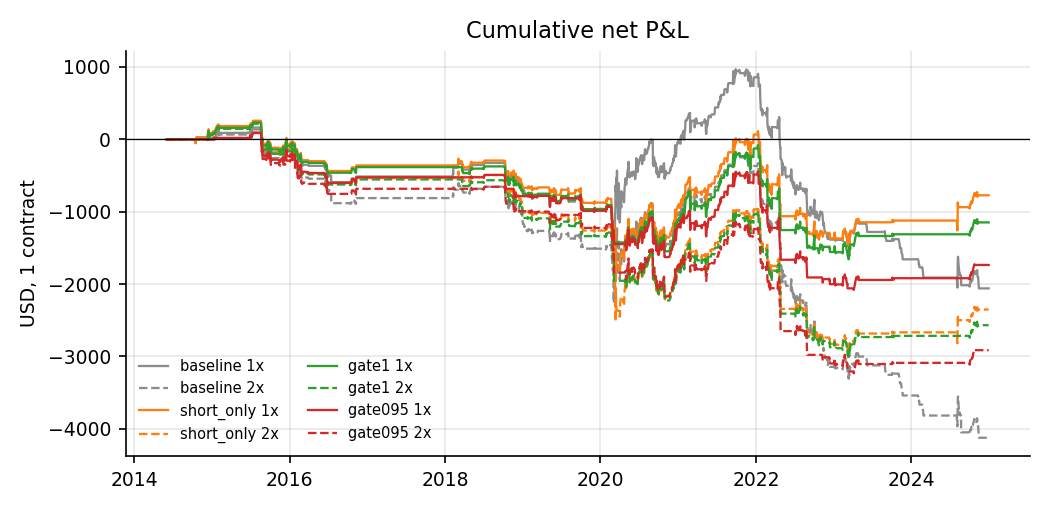
\includegraphics[width=0.92\linewidth]{figures/cum_pnl.png}\caption{Cumulative net P\&L, 1x solid and 2x dashed; baseline (live rules) grey}\end{figure}

\texttt{gate1} tracks \texttt{short\_\allowbreak{}only} almost everywhere: 90 of the reference's 100 round trips are unchanged, with the same entry and exit dates. The lines split in March-April 2020, where \texttt{gate1} skips the March crash loss but also misses the April rebound, and again in August 2024. \texttt{gate095} blocks far more entries and ends lowest at both spreads.

\begin{figure}[H]\centering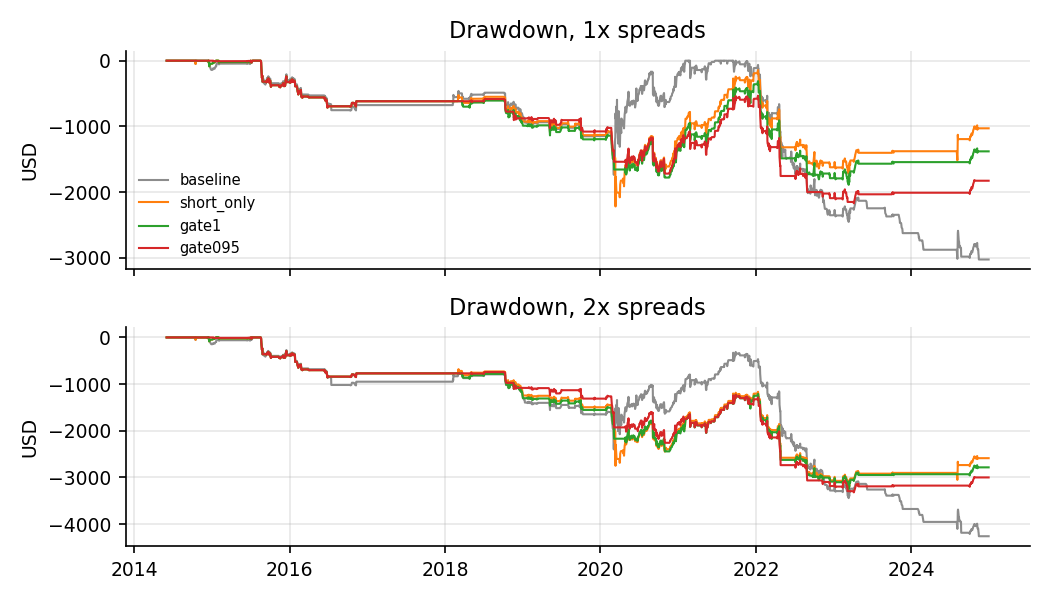
\includegraphics[width=0.92\linewidth]{figures/drawdown.png}\caption{Drawdown at 1x and 2x spreads}\end{figure}

At 1x the gate removes the sharp March 2020 dip, so its maximum drawdown is smaller (\$1,890 against \$2,220). At 2x the deepest point for both books comes in 2023, where they are nearly the same (\$3,251 against \$3,222).

\begin{figure}[H]\centering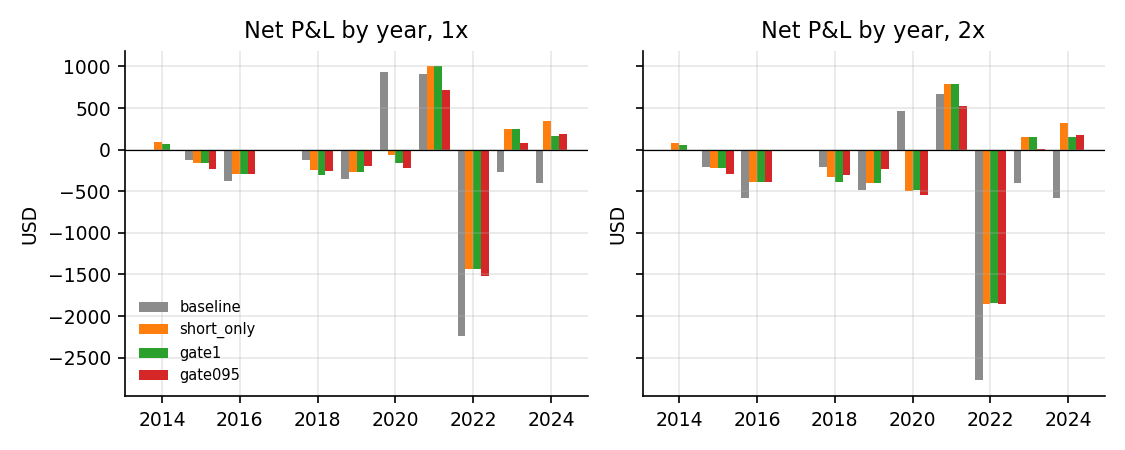
\includegraphics[width=0.92\linewidth]{figures/yearly.png}\caption{Net P\&L by year}\end{figure}

At 1x, \texttt{gate1} changes only five years against the reference: 2014 (\ensuremath{-}\$24), 2018 (\ensuremath{-}\$63), 2020 (\ensuremath{-}\$105), 2022 (+\$2) and 2024 (\ensuremath{-}\$185). Inside 2020 the effects nearly cancel: +\$415 in March, \ensuremath{-}\$393 in April. At 2x, 2020 is slightly positive (+\$12) and 2024 is again the largest cost (\ensuremath{-}\$168).

\begin{figure}[H]\centering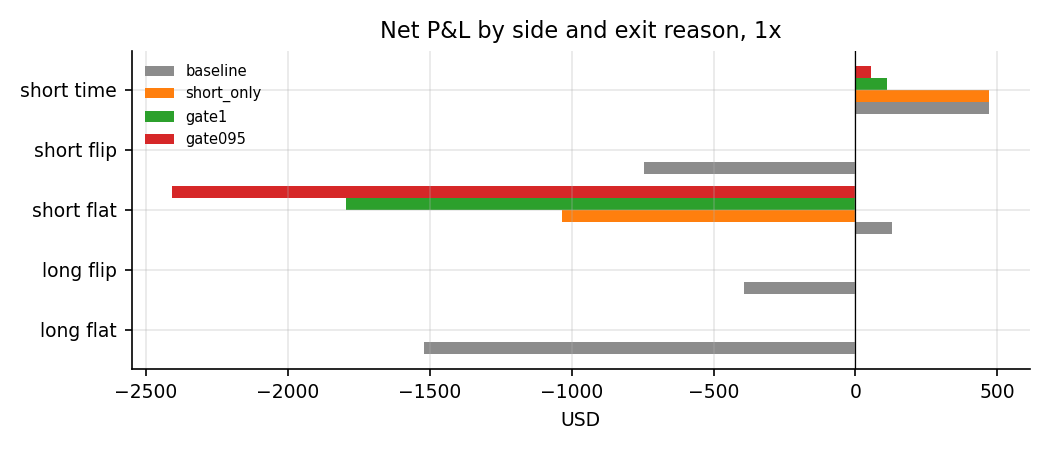
\includegraphics[width=0.92\linewidth]{figures/by_reason.png}\caption{Net P\&L by side and exit reason, 1x}\end{figure}

Most of the change shows up as flat exits. The reference's 87 flat exits lose \$1,032 net at 1x; \texttt{gate1}'s 80 lose \$1,795. Time exits fall from 13 (+\$470) to 12 (+\$112). The trades the gate removes are mostly short holds closed on a flat signal after a volatility spike, and on the round-trip ledger these were winners.

\begin{figure}[H]\centering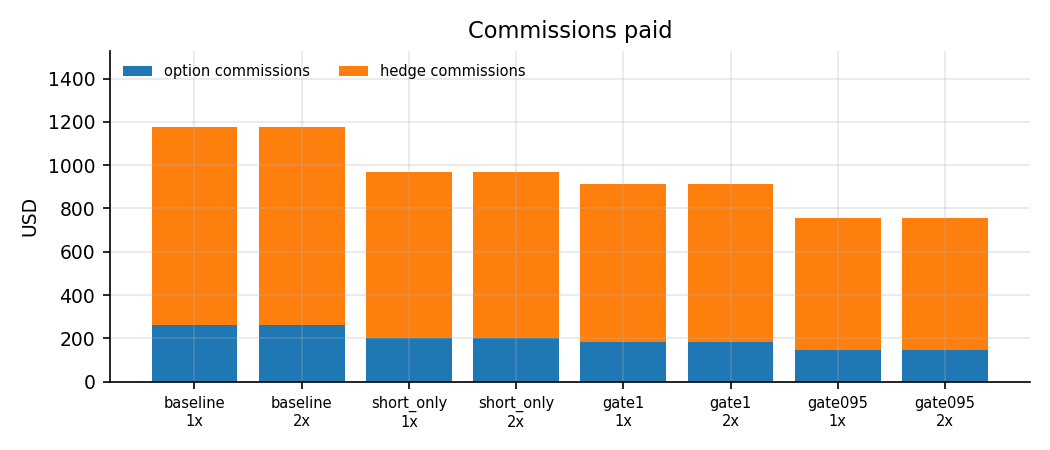
\includegraphics[width=0.92\linewidth]{figures/fees.png}\caption{Commissions paid}\end{figure}

Fewer trades means slightly lower commissions: \$58 less for \texttt{gate1} (8 fewer round trips, 42 fewer hedge orders) and \$216 less for \texttt{gate095}. That saving is small next to the P\&L the skipped trades would have earned.

\begin{figure}[H]\centering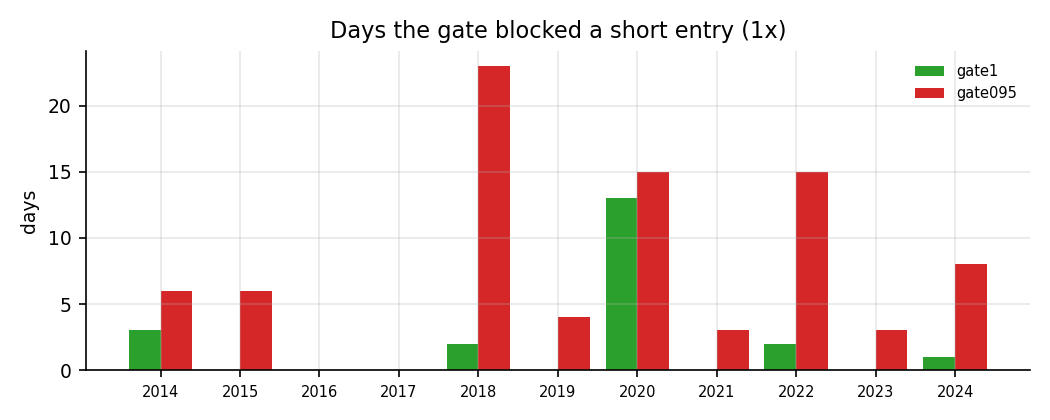
\includegraphics[width=0.92\linewidth]{figures/gate_per_year.png}\caption{Days the gate blocked a short entry, 1x}\end{figure}

\texttt{gate1} blocked shorts on 21 days. Thirteen fall in 2020: two in March, eight in April, and three in late October to early November. The rest: three in October 2014, two in 2018, two in October 2022 and one in August 2024. The curve closed inverted on 193 days of the window, but the gate only checks when the book is flat and the signal is short. \texttt{gate095} fires on 83 days, spread over every year except 2016-2017.

\begin{figure}[H]\centering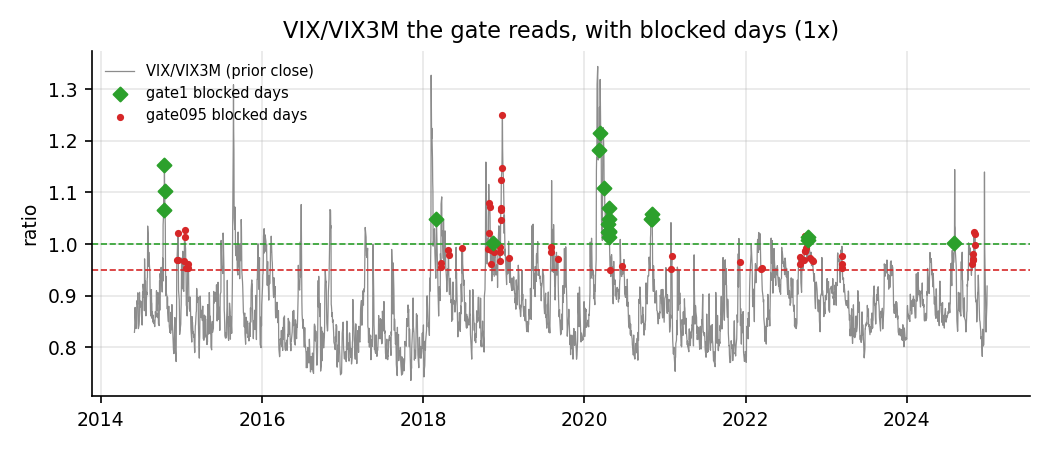
\includegraphics[width=0.92\linewidth]{figures/vix_ratio.png}\caption{VIX/\allowbreak{}VIX3M the gate reads (prior close), with blocked days marked; dashed lines are the two thresholds}\end{figure}

The blocked days sit on the inversions of October 2014, early and late 2018, March-April and October-November 2020, October 2022 and August 2024. Of the 193 inverted days, a short was already open on 83 and the signal was flat on 82 (the realized-vol forecast jumps with the spike, so VRP falls below the short band). Seven had no snapshot, which leaves the 21 blocked days. In August 2015 and late 2018 a short was usually already open; in February 2018 the signal stayed flat. The gate only blocks new entries; it never closes a short that is already open.

\begin{figure}[H]\centering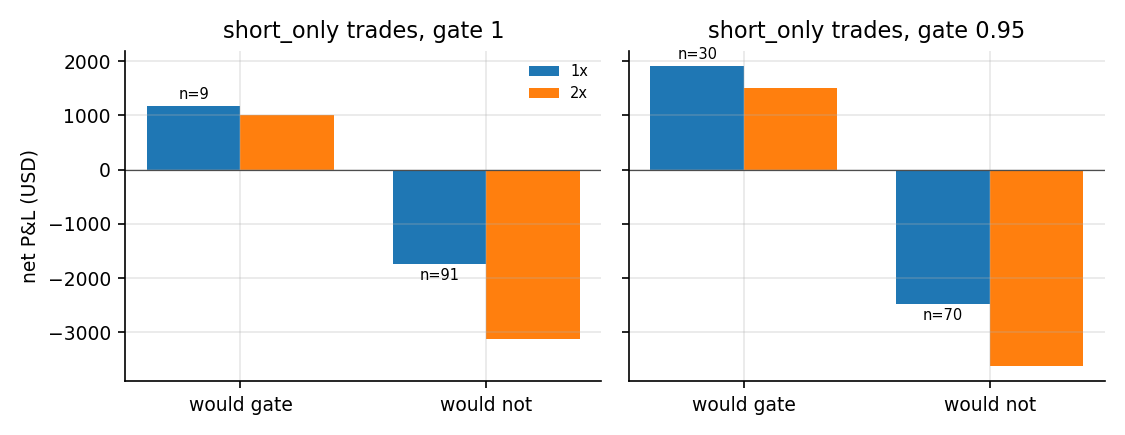
\includegraphics[width=0.92\linewidth]{figures/ref_split.png}\caption{Net P\&L of the reference's round trips whose entry day would or would not be gated}\end{figure}

This chart sorts the reference's own trades by the ratio at the prior close of their entry day. Nine entered on days \texttt{gate1} would gate. Together they made +\$1,170 net at 1x and +\$1,008 at 2x on the round-trip ledger (8 closed on a flat signal, 1 at 7 DTE). The other 91 lost \$1,732 at 1x. The 30 trades that \texttt{gate095} would gate made +\$1,915 at 1x. Shorts opened just after the curve inverts have been the reference's best trades, not its worst.

\section{Analysis}

\textbf{What the gate removes.} Against the reference, \texttt{gate1} drops 10 round trips and adds 2. All other 90 trades are identical. Nine of the dropped trades entered on gated days. The tenth is path dependence: once the gate cleared in late April 2020, \texttt{gate1} opened a short while the reference was still holding one, which displaced one of the reference's May 2020 entries. On the round-trip ledger, the dropped trades made +\$1,103 net at 1x (+\$1,185 before commissions), and the two new ones lost \$18. Five of the dropped trades are in 2020 (+\$841). Shorts opened right after a VIX spike collect inflated premium as volatility falls back, so they mostly close profitably on a flat signal. The 2026-10-07 proxy cards saw the same thing: many inverted days are good shorts.

\textbf{Where the tail cut comes from.} The cut is almost one episode. The reference's worst day is 2020-03-12 (\ensuremath{-}\$703 at 1x), inside a short opened on 2020-03-09 after the curve had closed inverted at 1.18. \texttt{gate1} blocks that entry and is flat through the crash, so its worst day is \ensuremath{-}\$328 (2020-09-04, shared with the reference). Setting the reference's daily P\&L to zero over 2020-03-09 to 03-17 moves its ES from \ensuremath{-}85.5 to \ensuremath{-}78.1. That is about three quarters of the gate's cut to \ensuremath{-}75.6. In 2014-2019 the gate improves ES by about 1\% (45.2 against 45.7). The 2020-2024 cut (16\% at 1x, 15\% at 2x) is mostly that one week. So the two ``less severe'' checks pass, but the first-half pass is marginal.

\textbf{P\&L bridge, \texttt{gate1} minus \texttt{short\_\allowbreak{}only}.}

\begin{center}\small
\begin{tabularx}{\linewidth}{>{\raggedright\arraybackslash}X l l}
\toprule
\textbf{} & \textbf{1x} & \textbf{2x} \\
\midrule
Round-trip P\&L before commissions & \ensuremath{-}1,173 & \ensuremath{-}1,016 \\
Commissions saved & +58 & +58 \\
Unattributed unwind residual & +741 & +742 \\
Net P\&L change (equity) & \ensuremath{-}374 & \ensuremath{-}217 \\
\bottomrule
\end{tabularx}
\end{center}

The residual is equity P\&L minus round-trip gross P\&L net of all commissions (the same definition as the other batch reports). Round trips value the closing hedge at the decision-time spot, while the equity curve books the share unwind at the fill-window price 15 minutes later. Usually the gap is noise; here it matters. Most of the +\$741 is one event: the reference's March 2020 short shows +\$28 on the round-trip ledger, but its 81-share unwind on 2020-03-17 filled about \$440 worse in total than the decision spot in a fast market. In equity terms, that trade cost the reference about \$415. The rest of the residual change nets out over April, May and November 2020 and August 2024. So the round-trip view overstates the gate's cost and the equity view, which the bar uses, is the right one. On equity, the gate still loses money because the April 2020 and August 2024 post-spike shorts it skips were profitable.

\textbf{Sensitivity.} \texttt{gate095} blocks 83 days, gets closer to the tail target (17.6\% at 1x, 17.7\% at 2x), and still misses 20\%. It costs about 2.6 times as much P\&L (\ensuremath{-}\$962 at 1x, \ensuremath{-}\$561 at 2x). At 1x it is worse than \texttt{gate1} in 2014, 2015 and 2020-2023, and better in 2018, 2019 and 2024. A lower threshold mostly removes more profitable post-spike shorts.

\section{Verdict}

\textbf{Failed} on the pre-registered bar: the tail cut is about 11-12\% (bar 20\%) at both spreads, and net P\&L falls at both spreads. The event floor was met (21 blocked days), so this is a real result, not an inconclusive one. On option P\&L with the live stops and exits, the gate does what the proxy cards suggested in one crash (March 2020). Everywhere else it removes the post-spike shorts that earn the most. Archive the gate as an entry filter for the short-only book. A follow-up idea that would need its own card: gate on the \emph{speed} of the inversion (for example, the first day the curve inverts, rather than any inverted day). The one loss avoided came at the start of a spike, while the gains given up came after it. That idea comes from these results, so it would be in-sample on this window.

\section{Caveats}

\begin{itemize}

\item \textbf{In-sample:} the idea comes from the 2026-10-16 desk discussion of the baseline on this window and from the 2026-10-07 proxy cards, whose data overlaps it. A failure here is still informative; a pass would have needed the hold-out.

\item \textbf{One episode:} about three quarters of the tail cut comes from one week in March 2020. With 21 blocked days and 10 changed trades, the result rests on a handful of events.

\item \textbf{Unwind residual:} a single fill-gap unwind in March 2020 moves the round-trip picture by about \$440. The spot comes from put-call parity on a 30-minute grid (10:15-15:45 ET), and fills use the next 15 minutes of trades, which is coarse in a crash.

\item \textbf{One contract:} the \$1 minimum per order is large relative to size.

\item \textbf{Spread model:} fitted on about two weeks of calm 2026 live quotes; the 2x run is the stress test.

\item \textbf{Data gaps:} R2 has no month-end weekdays, so about 3.3\% of scheduled times are skipped (89 times).

\end{itemize}

\section{Trials}

4 trials for this experiment (\texttt{gate1} and \texttt{gate095} at 1x and 2x, one run of \texttt{experiment.\allowbreak{}py}, commit fc6e788). The reference reuses the 2 registered \texttt{2026-\allowbreak{}10-\allowbreak{}16-\allowbreak{}short-\allowbreak{}only/\allowbreak{}short\_\allowbreak{}only} trials and was not rerun. Baseline trial 1 (2 runs) is shown for context. After the run, one chart was changed (the \texttt{gate1} markers in the VIX/\allowbreak{}VIX3M chart were hidden under \texttt{gate095}'s) and the figures were rebuilt with \texttt{-\allowbreak{}-\allowbreak{}report-\allowbreak{}only}, adding no trials. No registry rows are tagged \texttt{-\allowbreak{}dirty}. The pass bar was not changed.

\end{document}
